\documentclass{iopart}
\usepackage{arydshln}
\usepackage{multirow}
\usepackage{amsopn}
\usepackage{iopams}
\usepackage{graphicx}
\usepackage{bib/aas_macros}
\usepackage[colorlinks]{hyperref}
\input{ligo-acronyms/acronyms}

% From http://www.f.kth.se/~ante/latex.php
\setlength{\marginparwidth}{1.2in}
\let\oldmarginpar\marginpar
\renewcommand\marginpar[1]{\-\oldmarginpar[\raggedleft\footnotesize #1]%
{\raggedright\footnotesize #1}}

\DeclareMathOperator{\cov}{cov}
\DeclareMathOperator{\std}{std}
\DeclareMathOperator*{\argmin}{\arg\!\min}
\DeclareMathOperator*{\argmax}{\arg\!\max}

% Macros for collapsing sizes of things
% From TUGboat, Volume 22 (2001), No. 4
% http://www.tug.org/TUGboat/tb22-4/tb72perlS.pdf
\def\clap#1{\hbox to 0pt{\hss#1\hss}}
\def\mathllap{\mathpalette\mathllapinternal}
\def\mathrlap{\mathpalette\mathrlapinternal}
\def\mathclap{\mathpalette\mathclapinternal}
\def\mathllapinternal#1#2{\llap{$\mathsurround=0pt#1{#2}$}}
\def\mathrlapinternal#1#2{\rlap{$\mathsurround=0pt#1{#2}$}}
\def\mathclapinternal#1#2{\clap{$\mathsurround=0pt#1{#2}$}}

\begin{document}

\title[Rapid-response Bayesian sky localization]{WHOOMP! (There It Is) \\
Rapid Bayesian position reconstruction for gravitational\nobreakdashes-wave transients}
\author{Leo Singer and Larry R. Price}
\address{\acs{LIGO} Laboratory, California Institute of Technology, Pasadena, CA 91125, USA}
\ead{\mailto{leo.singer@ligo.org}, \mailto{larryp@caltech.edu}}

\begin{abstract}
\marginpar{Wrong emphasis? I like Larry's idea of having this paper discuss several different tiers of sky localization with increasing accuracy and latency.}%
Timely \acl{EM} follow\nobreakdashes-up of \acl{CBC} events detected by \acl{aLIGO} requires rapidly inferring the sky location from the \ac{GW} observations. Calculation of the posterior distribution of the sky location and intrinsic source parameters given the \ac{GW} strain takes hours with state\nobreakdashes-of\nobreakdashes-the\nobreakdashes-art \ac{MCMC} parameter estimation codes. By taking as the measurement not the \ac{GW} strain itself but the amplitude and \acl{TOA} of the putative signal at each detector, and by fixing the intrinsic source parameters, we have constructed a non-\ac{MCMC}, fully deterministic Bayesian parameter estimation algorithm that takes just seconds to produce sky maps of posterior probability.
\end{abstract}

Ground-based \ac{GW} interferometers are entering the advanced detector era, positioning themselves to make profound discoveries about the universe. The \ac{aLIGO} and Vigo detectors will be part of a worldwide network that also includes KAGRA and hopefully LIGO-India. Coalescing neutron star binaries are among the most likely sources, with 0.4\nobreakdashes--400 detections per year~\cite{rates}. In addition to being an efficient source of \acp{GW}, the \ac{NS} may be tidally shredded before merging, providing fuel for an electromagnetic counterpart. The short-lived accretion flow may power a collimated relativistic jet, resulting in a short \ac{GRB} and an X-ray afterglow if it is aligned with the line of sight. An optical afterglow may follow minutes to hours later as the jet plows into the interstellar medium. As surrounding neutron-rich ejecta decay radioactively, an optical `kilonova' may be visible after $\sim$1 day \cite{metzger:2010}. Finally, as the ejecta plow into the interstellar medium, a faint radio afterglow could occur on a timescale of weeks to years \cite{Nakar:2011cw}.

There is therefore a strong case for performing electromagnetic followups of these sources of \acp{GW}. Indeed, the final science run of the intitial LIGO and Virgo instruments saw the first joint search for \acp{GW} from compact binaries and their electromagnetic counterparts \cite{abadie2012first}.  As we prepare for the next generation of these searches there is a need for determining the location of the source as precisely as possible in as little time as possible.

In this paper we present a rapid and accurate method of sky localization that makes use of Bayesian methods. It differs from existing techniques in several important ways.  In the first place, we fix the intrinsic parameters to their \ac{ML} estimates, as provided by the detection pipeline.  This reduces the dimensionality of the parameter space we need to sample. In addition, the technique takes as its input the \ac{ML} estimates of the extrinsic parameters, instead of the $h(t)$ time series. This makes the likelihood itself much faster to evaluate. Finally, instead of of using \ac{MCMC} or some similar method for statistical sampling, we make use of a deterministic quadrature scheme. We call this technique \ac{BAYESTAR}%
%
\footnote{A pun on the Cylon battleships in the American television series Battlestar Galactica. The defining characteristic of the Cylons is that they repeatedly defeat humanity by using their superhuman information\nobreakdashes-gathering ability to coordinate overwhelming forces. The name also suggests that, like the Cylons, \ac{GW} detectors may some day rise against us humans.}%
%
\footnote{We do not like to mention the final `L' in the acronym, because then it would be pronounced BAYESTARL, which sounds stupid.}%
. It is unique in that in bridges the detection and parameter estimation of \ac{GW} signals, two tasks that have until now involved very different numerical methods and time scales. We expect that \ac{BAYESTAR} will take on a key role in observing \ac{CBC} events in both \ac{GW} and optical channels during the Advanced \ac{LIGO} era.

\section{Theory of \ac{GW} detection and parameter estimation}

In the frequency domain, the strain observed by a single \ac{GW} interferometer is
%
\begin{equation}\label{eq:signal-model}
	x_i (\omega) = h_i (\omega; \boldsymbol\theta) + n_i (\omega),
\end{equation}
%
where $h_i (\omega; \boldsymbol\theta)$ is the \ac{GW} signal given a parameter vector $\boldsymbol\theta$ that describes the \ac{GW} source, and $n_i (\omega)$ is that detector's \ac{WSS} Gaussian noise with one\nobreakdashes-sided \ac{PSD} $S_i(\omega) = E\left[\left|n_i(\omega)\right|^2\right]$. We shall denote the combined observation from a network of detectors as $\mathbf x (\omega) \equiv \{x_i (\omega)\}_i$.

The likelihood, or the probability of obtaining the observation $\mathbf x$ conditioned on the value of $\boldsymbol\theta$, is a product of Gaussian distributions:
%
\begin{equation}\label{eq:gaussian-likelihood}
	\mathcal{L}(\mathbf x; \boldsymbol\theta) = \prod_i p(x_i | \boldsymbol\theta)
		\propto \exp \left[
		- \frac{1}{2} \sum_i \int_0^\infty \frac{\left|x_i (\omega)
			- h_i(\omega; \boldsymbol\theta) \right|^2}{S_i(\omega)} \, d\omega
	\right].
\end{equation}

A \ac{CBC} source is specified by a vector of extrinsic parameters describing its position and orientation and intrinsic parameters describing the physical properties of the binary components:
%
\begin{equation}
    \boldsymbol\theta = \begin{array}{l@{}l}
            \left[
            \begin{array}{c}
                \alpha \\
                \delta \\
                D_\mathrm{L} \\
                t_\oplus \\
                u \\
                \psi \\
                \phi_c \\
                \hdashline[1pt/1pt]
                m_1 \\
                m_2 \\
                \mathbf S_1 \\
                \mathbf S_2
            \end{array}
            \right] &
            \begin{array}{l}
                \left.
                \begin{array}{p{4cm}}
                    right ascension \\
                    declination \\
                    luminosity distance \\
                    arrival time at geocenter \\
                    $\cos(\textrm{inclination angle})$ \\
                    polarization angle \\
                    coalescence phase \\
                    \hdashline[1pt/1pt]
                \end{array}
                \quad \right\} \textnormal{extrinsic parameters}, \boldsymbol\theta_\mathrm{ex} \\
                \left.
                \begin{array}{p{4cm}}
                    first component's mass \\
                    second component's mass \\
                    first component's spin \\
                    second component's spin
                \end{array}
                \quad \right\} \textnormal{intrinsic parameters}, \boldsymbol\theta_\mathrm{in}
            \end{array}
        \end{array}
\end{equation}
%
This list of parameters involves some simplifying assumptions. Eccentricity is omitted: although it does play a major role in the evolution and waveforms of \ac{NSBH} and \ac{BBH} sources formed by dynamical capture~\cite{PhysRevD.87.043004}, \ac{BNS} systems formed by binary stellar evolution should circularize due to tidal interaction~\cite{0004-637X-572-1-407} and later \ac{GW} emission~\cite{PhysRev.136.B1224} long before the inspiral enters \ac{LIGO}'s frequency range of $\sim$10\nobreakdashes--1000~kHz. Tidal deformabilities of the \acp{NS} are omitted because the signal imprinted by the companions' material properties is so small that it will only be detectable by an Einstein Telescope\nobreakdashes-class \ac{GW} observatory~\cite{PhysRevD.81.123016}. Furthermore, in \ac{GW} detection efforts, especially those focused on \ac{BNS} systems, the component spins $\mathbf{S}_1$ and $\mathbf{S}_2$ are often assumed to be nonprecessing and aligned with the system's total angular momentum and condensed to a single scalar parameter $\chi$, or even neglected entirely, $\mathbf{S}_1 = \mathbf{S}_2 = 0$.

Assuming circular orbits and no spin precession, we can write the \ac{GW} signal in each detector as a linear combination of two basis waveforms $h_0$ and $h_{\pi/2}$. For nonprecessing systems, $h = h_0$ and $h_{\pi/2}$ are approximately ``in quadrature'' in the same sense as the sine and cosine functions, being nearly orthogonal and out of phase by ${\pi/2}$ at all frequencies. In other words, $h_{\pi/2}(\omega) = i h_0(\omega)$ for all $\omega$. This linear combination isolates all dependence on the extrinsic parameters $\boldsymbol\theta_\mathrm{ex}$ into the coefficients and all dependence on the intrinsic parameters $\boldsymbol\theta_\mathrm{in}$ into the basis waveform,
%
\begin{eqnarray}\label{eq:full-signal-model}
	\fl h_i(\omega; \boldsymbol\theta) &=& e^{-i\omega t_\oplus}\frac{D_{1,i}}{D_\mathrm{L}}
	\left(\begin{array}{cc}
		F_{+,i}(\alpha, \delta, t_\oplus) \\
		F_{\times,i}(\alpha, \delta, t_\oplus)
	\end{array}\right)^\intercal
	\left(\begin{array}{cc}
		\cos{2\psi} & -\sin{2\psi} \\
		\sin{2\psi} & \cos{2\psi}
	\end{array}\right)
	\left(\begin{array}{cc}
		\frac{1}{2}\left(1+u^2\right) & 0 \\
		0 & u
	\end{array}\right) \nonumber\\\fl &\cdot&
	\left(\begin{array}{cc}
		\cos{2\phi_c} & -\sin{2\phi_c} \\
		\sin{2\phi_c} & \cos{2\phi_c}
	\end{array}\right)
	\left(\begin{array}{cc}
		1 \\
		i
	\end{array}\right) h(\omega; \boldsymbol\theta_\mathrm{in}).
\end{eqnarray}
%
This linear combination matches the conventions used in \cite{PhysRevD.83.084002}, and is the frequency-domain equivalent of their Equation~(2.8). The quantities $F_{+,i}$ and $F_{\times,i}$ are the dimensionless detector antenna factors, and depend on the orientation of detector $i$ as well as the sky location and sidereal time of the event, and are derived in~\cite{PhysRevD.63.042003}. The quantity $D_{1,i}$ is a fiducial distance at which detector $i$ would register SNR=1 for an optimally oriented binary (face\nobreakdashes-on, and in a direction perpendicular to the interferometer's arms),
%
\begin{equation}\label{eq:horizon}
D_{1,i} = 1 / \sigma_i, \qquad {\sigma_i}^2 = \int_0^\infty \frac{\left|h(\omega; \mathbf \theta)\right|^2}{S_i(\omega)} \,d\omega.
\end{equation}

More succinctly, we can write the signal received by detector $i$ in terms of observable extrinsic parameters $\boldsymbol\theta_i = (\rho_i, \gamma_i, \tau_i)$, the amplitude $\rho_i$, phase $\gamma_i$, and time delay $\tau_i$ on arrival at detector $i$,
%
\begin{equation}\label{eq:signal-model}
	h_i (\omega; \boldsymbol\theta_i, \boldsymbol\theta_\mathrm{in}) = h_i (\omega; \rho_i, \gamma_i, \tau_i, \boldsymbol\theta_\mathrm{in}) = \frac{\rho_i}{\sigma_i} e^{i (\gamma_i - \omega \tau_i)} h(\omega; \boldsymbol\theta_\mathrm{in}).
\end{equation}

The prevailing technique for detection of \acp{GW} from \acp{CBC} is to realize a \ac{MLE} from the likelihood in \Eref{eq:gaussian-likelihood} and the signal model in \Eref{eq:signal-model}. Concretely, this results in a bank of matched filters, or the cross-correlation between a template waveform and the incoming data stream,
%
\begin{equation}
y_i(\tau_i;\boldsymbol\theta_\mathrm{in}) = \frac{1}{\sigma_i (\boldsymbol\theta_\mathrm{in})} \int_0^\infty \frac{h^*(\omega; \boldsymbol\theta_\mathrm{in}) x_i(\omega) e^{i \omega \tau_i}}{S_i(\omega)} \,d\omega.
\end{equation}
%
The \ac{ML} point estimates of the signal parameters, $\mathrm{MLE}(\mathbf{x}) = \{\{ \hat{\boldsymbol\theta}_i \}_i, \hat{\boldsymbol\theta}_\mathrm{in}\} = \{\left\{ \hat\rho_i, \hat\gamma_i, \hat\tau_i \right\}_i, \hat{\boldsymbol\theta}_\mathrm{in}\}$, are given by
%
\begin{eqnarray}
	\hat{\boldsymbol\theta}_\mathrm{in}, \{\hat\tau_i\}_i
		&=& \argmax_{\boldsymbol\theta_\mathrm{in}, \{\hat\tau_i\}_i}
		\sum_i \left| y_i\left(\tau_i;
		\boldsymbol\theta_\mathrm{in}\right) \right|^2, \\
	\hat\rho_i &=& \left| y_i\left(\hat\tau_i;
		\hat{\boldsymbol\theta}_\mathrm{in}\right) \right|, \\
	\hat\gamma_i &=& \arg y_i\left(\hat\tau_i;
		\hat{\boldsymbol\theta}_\mathrm{in}\right).
\end{eqnarray}
%
A detection candidate consists of the set $\{\left\{ \hat\rho_i, \hat\gamma_i, \hat\tau_i \right\}_i, \hat{\boldsymbol\theta}_\mathrm{in}\}$. There are various ways to characterize the significance of a detection candidate, but in Gaussian noise the combined SNR $\hat\rho_\mathrm{c}$ suffices,
%
\marginpar{What is the least that I can get away with saying about false alarm rate estimation and likelihood ratios?}%
%
\begin{equation}
	\hat\rho_\mathrm{c} = \sqrt{\sum_i {\hat\rho_i}^2}.
\end{equation}

\subsection{Bayesian probability and parameter estimation}

In the Bayesian framework, the parameters are inferred from the data by forming the posterior distribution, $p(\boldsymbol\theta|\mathbf x)$, which describes the probability of the parameters given the observations. Bayes' rule relates the likelihood $p(\mathbf x|\boldsymbol\theta)$ to the posterior $p(\boldsymbol\theta|\mathbf x)$,
%
\begin{equation}\label{bayes}
p(\boldsymbol\theta|\mathbf x) = \frac{p(\mathbf x|\boldsymbol\theta) p(\boldsymbol\theta)}{p(\mathbf x)},
\end{equation}
%
introducing the prior distribution $p(\boldsymbol\theta)$ which encapsulates previous information about the paramters (for example, arising from earlier observations or from known physical bounds on the parameters), and the evidence $p(\mathbf x)$ which can be thought of as a normalization factor or as describing the parsimoniousness of the model.

The choice of prior is open to one's astrophysical preconceptions, but during \ac{S6} when \ac{LIGO}'s Bayesian \ac{CBC} parameter estimation pipelines were pioneered, the prior was taken to be isotropic in sky location and binary orientation, and uniform in volume, arrival time, and the component masses~\cite{2013arXiv1304.1775T}.

In Bayesian inference, although it is often easy to write down the likelihood or even the full posterior in closed form, usually one is interested in only a subset $\boldsymbol\beta$ of all of the model's parameters, the others $\boldsymbol\lambda$ being nuisance parameters. In this case, we integrate away the nuisance parameters, forming the marginal posterior
%
\begin{equation}\label{eq:marginal-posterior}
	p(\boldsymbol\beta|\mathbf x) = \int \frac{p(\mathbf x|\boldsymbol\beta,\boldsymbol\lambda) p(\boldsymbol\beta,\boldsymbol\lambda)}{p(\mathbf x)} \,d\boldsymbol\lambda
\end{equation}
%
with $\boldsymbol\theta = (\boldsymbol\beta, \boldsymbol\lambda)$. For instance, for the purpose of locating a \ac{GW} source on the sky, all parameters but $(\alpha, \delta)$ are nuisance parameters.

Bayesian parameter estimation has many advantages, including broad generality and the ability to make probabilistically meaningful statements even with very low \ac{SNR} measurements. However, in problems of even modest complexity, the marginalization step involves many-dimensional, ill-behaved integrals. The powerful \ac{MCMC} integration technique has become almost synonymous with Bayesian inference. Though powerful, \ac{MCMC} is inherently non-deterministic and resistant to parallelization, as well as (at least historically) slow. With the most sophisticated \ac{CBC} parameter estimation codes, it still takes days to process a single event. This delay is undesirable for planning targeted \ac{EM} follow\nobreakdashes-up searches of \ac{LIGO} events.

In what follows, we propose a complementary rapid parameter estimation scheme that can produce reliable positions estimates within minutes of a detection. We can even use our scheme to speed up the full \ac{MCMC} analysis and make the refined parameter estimates available more quickly. The key difference is that we start not from the \ac{GW} signal itself, but from the point parameter estimates from the detection. By harnessing the detection pipeline in this manner, we arrive at a simpler Bayesian problem that is amenable to straightforward, deterministic, numerical quadrature.

\section{Measurement uncertainty}

For the purpose of rapid sky localization, we assume that we do not have access to the \ac{GW} data $\mathbf{x}$ itself, and that our only contact with it is through the ML parameter estimates $\{\left\{ \hat\rho_i, \hat\gamma_i, \hat\tau_i \right\}_i, \hat{\boldsymbol\theta}_\mathrm{in}\}$. Although this is a significant departure from conventional GW parameter estimation techniques, we can still apply the full Bayesian machinery of \Eref{eq:marginal-posterior} to compute a posterior distribution for the sky location.

\marginpar{This paragraph might make more sense in a conclusion.}%
%
There are many practical advantages of doing so. For one, there are difficulties in synchronously gathering together the calibrated GW strain data, auxiliary instrument channels, and data quality vetoes from all of the sites. The data consumed by the real\nobreakdashes-time detection pipeline are not necessarily final. Longer\nobreakdashes-running follow\nobreakdashes-up analyses can benefit from offline calibration, whereas the rapid sky localization need not re\nobreakdashes-analyze the online data. Moreover, the dimensionality of the problem is greatly reduced, and the problem becomes computationally easier.

\subsection{Fisher matrix: single detector}

To treat the ML estimates as measurements in and of themselves, we need to work out their likelihood, marginalized over the GW signal $\mathbf{x}$,
%
\begin{equation}\label{eq:detection-candidate-likelihood}
	p\left(\{\hat{\boldsymbol\theta}_i\}_i,
		\hat{\boldsymbol\theta}_\mathrm{in}
	\middle| \boldsymbol\theta\right)
	\propto \int\limits_{\mathclap{\mathbf{x} | \mathrm{MLE}(\mathbf{x}) =
		\{\{\hat{\boldsymbol\theta}_i\}_i,
		\hat{\boldsymbol\theta}_\mathrm{in}\}}}
	p(\mathbf{x} | \boldsymbol\theta) \, p(\boldsymbol\theta)
	\, d\mathbf{x}
\end{equation}
%
The integral above could be written in terms of the matched filter signals $\left\{y_i\right\}_i$, such that $y_i\left(\hat\tau_i, \hat{\boldsymbol\theta}_\mathrm{in}\right) = \hat\rho_i e^{\hat\gamma_i}$ and $\forall t$, $\left|y_i(t, \boldsymbol\theta_\mathrm{in})\right| \leq \hat\rho_i$. The combination of the nontrivial integration limits and the Fourier transform in the matched filter seem like a problem for direct evaluation.

However, even without directly evaluating the distribution of the \ac{ML} estimator, we know many of its properties. The \ac{CRLB} gives its covariance in the asymptotic limit of high \ac{SNR}. The \ac{CRLB} has been widely applied in \ac{GW} data analysis \cite{fairhurst:2009}. We will momentarily consider the likelihood for a single detector:
%
\begin{equation}\label{eq:gaussian-likelihood-spa}
	\mathcal{L}\left(x_i; \rho_i, \gamma_i, \tau_i,
		\boldsymbol\theta_\mathrm{in}\right)
	\propto \exp \left[
		- \frac{1}{2} \int_0^\infty \frac{\left|x_i (\omega)
			- h_i\left(x_i; \rho_i, \gamma_i, \tau_i,
				\boldsymbol\theta_\mathrm{in}\right)
		\right|^2}{S_i(\omega)} \, d\omega
	\right],
\end{equation}
%
with $h_i(\omega; \rho_i, \gamma_i, \tau_i, \boldsymbol\theta_\mathrm{in})$ given by \Eref{eq:signal-model}.

The Fisher information matrix for a measurement $x$ described by the unknown parameter vector $\boldsymbol{\theta}$ is
%
\begin{equation}\label{eq:general-fisher-matrix}
	\mathcal{I}_{jk} = \mathrm{E} \, \left[
		-\frac{\partial^2 \log
			\mathcal{L}(x_i ; \boldsymbol\theta)}
			{\partial \theta_j \theta_k}
	\right].
\end{equation}
%
This equation involves double derivatives, but substantial simplification is possible when---as in this case---the likelihood is Gaussian:
%
\begin{equation}\label{eq:gaussian-fisher-matrix}
	\mathcal{I}_{jk} = \int_0^\infty \Re \left[
        \left(\frac{\partial h_i}{\partial \theta_j}\right)^*
        \left(\frac{\partial h_i}{\partial \theta_k}\right)
	\right] \frac{1}{S_i(\omega)} \, d\omega.
\end{equation}
%
This form is more useful because it involves only first derivatives, and of the signal $h (\omega)$ rather than the entire observation $x (\omega)$. In terms of the $k$th \ac{SNR}-weighted moment of angular frequency,
%
\begin{equation}\label{eq:angular-frequency-moments}
    {\overline{\omega^k}}_i =
        \left[ \int_0^\infty \frac{|h (\omega)|^2}{S_i(\omega)} \omega^k \, d\omega \right]
        \left[ \int_0^\infty \frac{|h (\omega)|^2}{S_i(\omega)} \, d\omega \right]^{-1},
\end{equation}
%
the Fisher matrix for the signal in the $i$th detector is
%
\begin{equation}
	\mathcal{I}_i = \left(
		\begin{array}{cc}
			\mathcal{I}_{\boldsymbol\theta_i,\boldsymbol\theta_i} &
			\mathcal{I}_{\boldsymbol\theta_i,\boldsymbol\theta_\mathrm{in}} \\
			{\mathcal{I}_{\boldsymbol\theta_i,\boldsymbol\theta_\mathrm{in}}}^\intercal &
			{\rho_i}^2 \mathcal{I}_{\boldsymbol\theta_\mathrm{in},\boldsymbol\theta_\mathrm{in}}
		\end{array}
	\right)
\end{equation}
%
where
%
\begin{equation}\label{eq:fisher-matrix}
	\mathcal{I}_{\boldsymbol\theta_i,\boldsymbol\theta_i} = \bordermatrix{
        ~ & \rho_i & \gamma_i & \tau_i \cr
        \rho_i & 1 & 0 & 0 \cr
        \gamma_i & 0 & {\rho_i}^2 & -{\rho_i}^2 {\overline{\omega}}_i \cr
        \tau_i & 0 & -{\rho_i}^2 {\overline{\omega}}_i & {\rho_i}^2 {\overline{\omega^2}}_i
    }.
\end{equation}
%
To lowest post\nobreakdashes-Newtonian order, the intrinsic parameters affect the phase evolution but not the amplitude evolution, so for BNS systems we can assume $\mathcal{I}_{\rho_i,\boldsymbol\theta_\mathrm{in}} \approx 0$.
%
\marginpar{Show this?}%
%
When we form the Fisher matrix for the whole network, if the detectors all have the same noise \acp{PSD}, $S_1(\omega) = S_1(\omega) = \cdots = S_n(\omega) \equiv S(\omega)$, then we can change variables from phases and times on arrival $\left\{\gamma_i, \tau_i\right\}_i$ to appropriate differences between them, in order to cancel out all off-diagonal terms between the intrinsic and extrinsic parameters. Because all existing ground-based GW detectors have similar bandpasses, we restrict all of our further attention to just the extrinsic part of the Fisher matrix, $\mathcal{I}_{\boldsymbol\theta_i,\boldsymbol\theta_i}$.

\subsection{\ac{CRLB} and physical interpretation}

If $\hat{\boldsymbol\theta}$ is an unbiased estimator of $\boldsymbol\theta$, $\tilde{\boldsymbol\theta} = \hat{\boldsymbol\theta} - \boldsymbol\theta$ is the measurement error, and $\Sigma = \mathrm{E} \, [\tilde{\boldsymbol\theta}\tilde{\boldsymbol\theta}^\intercal]$ is the covariance of the measurement error, then the \ac{CRLB} says that $\Sigma \geq \mathcal{I}^{-1}$, in the sense that $\left(\Sigma - \mathcal{I}^{-1}\right)$ is positive semi\nobreakdashes-definite. Specifically, for our likelihood, the \ac{CRLB} implies that
%
\begin{equation}\label{eq:covariance-matrix}
    \cov{
        \left(
        \begin{array}{c}
            \tilde{\rho}_i \\
            \tilde{\gamma}_i \\
            \tilde{\tau}_i
        \end{array}
        \right)
    } \geq \mathcal{I}^{-1} = \left(
        \begin{array}{ccc}
            1 & 0 & 0 \\
            0 & {\rho_i}^2 {\overline{\omega^2}}_i/{\omega_{\mathrm{rms},i}}^2 & {\rho_i}^2 {\overline{\omega}}_i/{\omega_{\mathrm{rms},i}}^2 \\
            0 & {\rho_i}^2 {\overline{\omega}}_i/{\omega_{\mathrm{rms},i}}^2 & {\rho_i}^2/{\omega_{\mathrm{rms},i}}^2
        \end{array}
    \right)
\end{equation}
%
where ${\omega_{\mathrm{rms},i}}^2 = {\overline{\omega^2}}_i - {{\overline{\omega}}_i}^2$. Reading off the $\tau \tau$ element of the covariance matrix reproduces the timing accuracy in Equation~(24) of \cite{fairhurst:2009},
%
\begin{equation}\label{eq:timing-crlb}
    \std \left(\hat{\tau}_i - \tau_i \right) \geq \sqrt{\left(\mathcal{I}^{-1}\right)_{\tau\tau}} = \frac{\rho_i}{\omega_{\mathrm{rms},i}}.
\end{equation}
%
Furthermore, the Fisher matrix in \Eref{eq:fisher-matrix} is block diagonal, which implies that estimation errors in the signal amplitude $\rho$ are uncorrelated with the phase $\gamma$ and time $\tau$. A sequence of two changes of variables lends some physical interpretation to the nature of the coupled estimation errors in $\gamma$ and $\tau$.

First, we put the phase and time on the same footing by measuring the time in units of $1 / \sqrt{\overline{\omega^2}}$ with a change of variables from $\tau$ to $\gamma_\tau = \sqrt{\overline{\omega^2}} \tau$:
%
\begin{equation}
    \mathcal{I}' = \bordermatrix{
        ~ & \rho_i & \gamma_i & \gamma_{\tau,i} \cr
        \rho_i & 1 & 0 & 0 \cr
        \gamma_i & 0 & {\rho_i}^2 & -{\rho_i}^2\frac{{\overline{\omega}}_i}{\sqrt{{\overline{\omega^2}}_i}} \cr
        \gamma_{\tau,i} & 0 & -{\rho_i}^2\frac{{\overline{\omega}}_i}{\sqrt{{\overline{\omega^2}}_i}} & {\rho_i}^2
    }.
\end{equation}
%
The second change of variables, from $\gamma$ and $\gamma_\tau$ to $\gamma_\pm = \frac{1}{\sqrt{2}}(\gamma \pm \gamma_\tau)$, diagonalizes the Fisher matrix:
%
\begin{equation}\label{eq:fisher-matrix-extrinsic-one-detector}
    \mathcal{I}'' = \bordermatrix{
        ~ & \rho_i & \gamma_{+,i} & \gamma_{-,i} \cr
        \rho_i & 1 & 0 & 0 \cr
        \gamma_{+,i} & 0 & \left(1 - \frac{\overline{\omega}_i}{\sqrt{\overline{\omega^2}_i}}\right){\rho_i}^2 & 0 \cr
        \gamma_{-,i} & 0 & 0 & \left(1 + \frac{\overline{\omega}_i}{\sqrt{\overline{\omega^2}_i}}\right){\rho_i}^2
    }.
\end{equation}
%
Thus, in the appopriate time units, the \textit{sum and difference} of the phase and time of the signal are measured independently.

\section{The \ac{BAYESTAR} likelihood}

Although we may not be able to compute the detection candidate likelihood, \Eref{eq:detection-candidate-likelihood}, directly, we can make an educated guess that has many properties in common with it. Any valid approximate likelihood must have the same Fisher matrix \Eref{eq:fisher-matrix-extrinsic-one-detector}. It must also have the same limiting behavior: it should be periodic in the phase error $\tilde{\gamma}_i$ and go to zero as $\tilde{\tau}_i \rightarrow \pm \infty$, $\hat{\rho}_i \rightarrow 0$, or $\hat{\rho}_i \rightarrow \infty$. Additionally, when $\tilde{\tau}_i = 0$, the distribution of ${\hat{\rho}_i}^2$ should reduce to a noncentral $\chi^2$ distribution with two degrees of freedom, centered about ${\rho_i}^2$, because the complex matched filter time series $y_i(t)$ is Gaussian.

These conditions could be satisfied by realizing a multivariate Gaussian distribution with covariance matrix $\Sigma = \mathcal{I}^\intercal$, and then replacing individual terms of the form $-\tilde{\theta}^2/2$ with $\cos{\tilde{\theta}}$.

\marginpar{Actually, this does not give exactly the same Fisher matrix. Explain.}%
%
Another way is to plug the signal model from \Eref{eq:signal-model} \emph{evaluated at the ML parameter estimates} into the single-detector likelihood in \Eref{eq:gaussian-likelihood-spa}:
%
\begin{eqnarray*}
	\fl p\left(\hat{\boldsymbol\theta}_i \middle| \boldsymbol\theta \right)
	&:=&
	p\left(x_i(\omega) = h_i(\omega; \hat{\boldsymbol\theta}_i)
		\middle| \boldsymbol\theta \right)
	\\\fl
	&\propto& \exp \left[
		- \frac{1}{2} \int_0^\infty \frac{\left|
			\frac{\hat{\rho}_i}{\sigma_i(\hat{\boldsymbol\theta}_\mathrm{in})} e^{i (\hat\gamma_i - \omega \hat\tau_i)} h(\omega; \hat{\boldsymbol\theta}_\mathrm{in})
			- \frac{\rho_i}{\sigma_i(\boldsymbol\theta_\mathrm{in})} e^{i (\gamma_i - \omega \tau_i)} h(\omega; \boldsymbol\theta_\mathrm{in})
		\right|^2}{S_i(\omega)} \, d\omega
	\right].
\end{eqnarray*}
%
If we assume that $\hat{\boldsymbol\theta}_\mathrm{in} = \boldsymbol\theta_\mathrm{in}$, then this reduces to
%
\begin{equation}\label{eq:autocor-likelihood}
	p\left(\hat\rho_i, \hat\gamma_i, \hat\tau_i
		\middle| \rho_i, \gamma_i, \tau_i \right) \propto
	\exp \left[ - \frac{1}{2}{\hat\rho_i}^2 - \frac{1}{2}{\rho_i}^2
		+ \hat\rho_i \rho_i \Re \left\{ e^{i \tilde{\gamma}_i} a_i^*(\tilde{\tau}_i)
		\right\}
	\right]
\end{equation}
%
with $\tilde{\gamma}_i = \hat\gamma_i - \gamma_i$, $\tilde{\tau}_i = \hat\tau_i - \tau_i$, and the template's autocorrelation function $a_i(t; \boldsymbol\theta_\mathrm{in})$ defined as
%
\begin{equation}
	a_i(t; \boldsymbol\theta_\mathrm{in}) := \frac{1}{{{\sigma_i}^2(\boldsymbol\theta_\mathrm{in})}} \int_0^\infty \frac{\left| h(\omega; \hat{\boldsymbol\theta}_\mathrm{in})\right|^2}{S_i(\omega)} e^{i \omega t} \,d\omega.
\end{equation}

To assemble the joint likelihood for the whole network, we just form the product from the individual detectors:
%
\begin{equation}
	\fl p\left(\left\{\hat\rho_i, \hat\gamma_i, \hat\tau_i\right\}_i
		\middle| \left\{\rho_i, \gamma_i, \tau_i\right\}_i \right) \propto
	\exp \left[ - \frac{1}{2} \sum_i {\hat\rho_i}^2 - \frac{1}{2} \sum_i {\rho_i}^2
		+ \sum_i \hat\rho_i \rho_i \Re \left\{ e^{i \tilde{\gamma}_i} a^*(\tilde{\tau}_i)
		\right\}
	\right].
\end{equation}
%
To marginalize over the coalescence phase, we can insert an arbitrary nuisance phase $\eta$ by making the replacement $\tilde{\gamma}_i \rightarrow \tilde{\gamma}_i + \eta$. Then integrating over $\eta$ from $0$ to $2\pi$ and suppressing normalization factors, we get the \ac{BAYESTAR} likelihood
%
\marginpar{Different symbol? Is $\mathcal{L}_\mathrm{BAYESTAR}$ too grandiose?}
%
\begin{equation}
	\mathcal{L}_\mathrm{BAYESTAR} = \exp \left[ - \frac{1}{2} \sum_i {\rho_i}^2 \right] I_0 \left[
		\left| \sum_i \hat\rho_i \rho_i e^{i \tilde{\gamma}_i} a_i^*(\tilde{\tau}_i)
		\right|
	\right],
\end{equation}
%
where $I_0$ is a modified Bessel function of the first kind.

\subsection{Properties}

Fisher matrix elements of \Eref{eq:autocor-likelihood}, with detector subscript suppressed:
%
\begin{eqnarray}
	\nonumber
	\mathcal{I}_{\rho\rho} &=& 1 \\
	\nonumber
	\mathcal{I}_{\rho\gamma} &=& 0 \\
	\nonumber
	\mathcal{I}_{\rho\tau} &=& 0 \\
	\mathcal{I}_{\gamma\gamma} &=& \rho^2
		\int_{-\infty}^\infty \left|a(t)\right|^2 w(t; \rho) dt \\
	\mathcal{I}_{\tau\tau} &=& -\rho^2
		\int_{-\infty}^\infty \Re\left[a^*(t) a''(t)\right] w(t; \rho) dt \\
	\mathcal{I}_{\gamma\tau} &=& -\rho^2
		\int_{-\infty}^\infty \Im\left[a^*(t) a'(t)\right] w(t; \rho) dt \\
	\nonumber\textrm{where} && \\
	\nonumber
	a'(t) &=& \frac{\partial a}{\partial t} \\
	\nonumber
	a''(t) &=& \frac{\partial^2 a}{\partial t^2} \\
	\nonumber
	w(t; \rho) &=& \frac{
		\displaystyle
		\exp\left[\frac{\rho^2}{4}\left|a(t)\right|^2\right]
		\left(
		I_0\left[\frac{\rho^2}{4}\left|a(t)\right|^2\right] +
		I_1\left[\frac{\rho^2}{4}\left|a(t)\right|^2\right]
		\right)
	}{
		\displaystyle
		2 \int_{-\infty}^\infty
		\exp\left[\frac{\rho^2}{4}\left|a(t')\right|^2\right]
		I_0\left[\frac{\rho^2}{4}\left|a(t')\right|^2\right]
		dt'
	}.
\end{eqnarray}
%
Matrix elements that are not listed have values that are implied by the symmetry of the Fisher matrix. Note that the minus signs are correct but a little confusing: despite them, ${I}_{\gamma\gamma}, {I}_{\tau\tau} \geq 0$ and ${I}_{\gamma\tau} \leq 0$.

If we can show that the common factor approaches a delta function, $w(t; \rho) \rightarrow \delta(t)$ as $\rho \rightarrow \infty$, then the Fisher matrix approaches \Eref{eq:fisher-matrix} as $\rho \rightarrow \infty$. Certainly it behaves very much like a delta function. The Bessel functions asymptotically approach:
%
\begin{equation*}
	I_0(x), I_1(x) \rightarrow \frac{e^x}{\sqrt{2 \pi x}}
	\textrm{ as } x \rightarrow \infty.
\end{equation*}
%
For large $\rho$, it seems like we could write:
%
\begin{equation*}
	w(t; \rho) \rightarrow \frac{
		\displaystyle
		\exp\left[\frac{\rho^2}{2}|a(t)|^2\right]
	}{
		\displaystyle
		\int_{-\infty}^\infty \exp\left[\frac{\rho^2}{2}|a(t')|^2\right] dt'
	}
	\textrm{ as } \rho \rightarrow \infty.
\end{equation*}

\section{The \ac{BAYESTAR} algorithm}

\subsection{Likelihood}

\subsection{Prior}

We have no explicit prior on the intrinsic parameters; in our analysis they are fixed at their \ac{ML} estimates, $\hat{\boldsymbol\theta}$. The distance prior is given by a user-selected power of distance, ${D_\mathrm{L}}^m$, where $m=2$ for a prior that is uniform in volume, and $m=-1$ for a scale-invariant prior that is uniform in $\log D_\mathrm{L}$. The priors are bounded as follows:
%
\marginpar{Need to discuss $D_{\mathrm{L},\mathrm{min}}$, $D_{\mathrm{L},\mathrm{max}}$, and how they are selected automatically if the user does not provide them.}%
%
\begin{eqnarray*}
	D_\mathrm{L} &\in& [D_{\mathrm{L},\mathrm{min}}, D_{\mathrm{L},\mathrm{max}}] \\
	t_\oplus &\in& [-\infty, \infty] \\
	u &\in& [-1, 1] \\
	\psi &\in& [0, \pi/2)
\end{eqnarray*}

\subsection{Adaptive resolution}

The \ac{TOA}\nobreakdashes-only posterior in \Eref{eq:toa-posterior} is numerically trivial to evaluate because it involves no numerical integrals. However, as we will see in the next section, the \ac{SNR}\nobreakdashes-only posterior is numerically expensive.

\marginpar{Clumsy prose.}%
We evaluate the \ac{TOA}\nobreakdashes-only posterior at the centers of \ac{HEALPix} pixels at the lowest possible resolution. Then, we increase the resolution until 99.99\% of the \ac{TOA}\nobreakdashes-only posterior is contained within at least 3072 pixels. The numerically expensive \ac{SNR} integrals are done only for the pixels that comprise the 99.99th percentile at this resolution. All other pixels are set to zero.

\subsection{Posterior}

\begin{eqnarray}
    p(
		\mathbf{n} |
        \hat{\tau}_1, \hat{\tau}_2, &\dots, \hat{\tau}_N,
        \hat{\rho}_1, \hat{\rho}_2, \dots, \hat{\rho}_N) \nonumber\\
    &= p(\mathbf{n} |
        \hat{\tau}_1, \hat{\tau}_2, \dots, \hat{\tau}_N) \nonumber\\
        &\times
        p(\mathbf{n} |
		\hat{\rho}_1, \hat{\rho}_2, \dots, \hat{\rho}_N
    )
\end{eqnarray}
%
where
%
\begin{equation*}
	\fl
    p(\mathbf{n} |
	\hat{\rho}_1, \hat{\rho}_2, \dots, \hat{\rho}_N)
	\propto
	\int_0^\frac{\pi}{2}
	\int_0^1
	\int_{D_{\mathrm{L},\mathrm{min}}}^{D_{\mathrm{L},\mathrm{max}}}
	\exp \left[
	        -\frac{1}{2} \sum_{i=1}^N \left(\hat{\rho}_i - \rho_i(\mathbf{n}, D_\mathrm{L}, u, \psi) \right)^2
	    \right]
	{D_\mathrm{L}}^m
	\,dD_\mathrm{L}
	\,du
	\,d\psi.
\end{equation*}

The marginalization over $D_\mathrm{L}$, $u$, and $\psi$ must be done numerically. The outermost integration is over $u$ and $\psi$, and is done with Newton\nobreakdashes--Cotes by evaluating $\mathcal{L}_\mathrm{SNR}$ on a regular lattice in $u$ and $\psi$.

\begin{figure}
    \caption{\label{fig:radial_integrand}Illustration of initial subdivisions for distance integration scheme. Distance increases from left to right. In the color version, the left\nobreakdashes-hand tail, the left\nobreakdashes- and right\nobreakdashes-hand sides of the maximum likelihood peak, and the right\nobreakdashes-hand tail, are colored cyan, red, green, and blue, respectively.}
    \begin{center}
        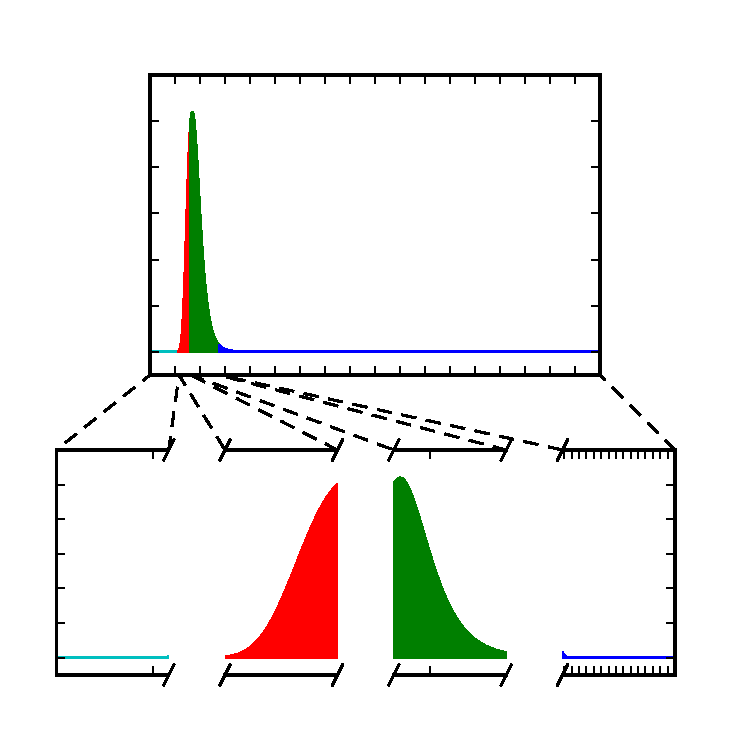
\includegraphics{radial_integrand}
    \end{center}
\end{figure}

The innermost integration is over $D_\mathrm{L}$ and is performed using adaptive Gaussian quadrature, but with a twist that speeds up convergence. As in many parameter estimation problems, the integrand may be sharply peaked, and any generic adaptive integration scheme may take a long time to find the peak. Before evaluating each inner integral over $D_\mathrm{L}$, the quantities $A=-\frac{1}{2} \sum_i {\rho_i}^2$ and $B=\sum_i \rho_i \hat\rho_i$ are pre\nobreakdashes-calculated so that the integrand can be written as
%
\begin{equation*}
	\exp\left(\frac{A}{{D_\mathrm{L}}^2} + \frac{B}{D_\mathrm{L}}\right) {D_\mathrm{L}}^m.
\end{equation*}
%
Then, we see that the likelihood $\exp(A {D_\mathrm{L}}^{-2} + B {D_\mathrm{L}}^{-1})$ is maximized when $D_\mathrm{L} = D_{\mathrm{L},0} = -2A/B$. The likelihood takes on a factor $\eta$ (say, $\eta=0.01$) of its maximum value when
%
\begin{equation}
	D_\mathrm{L} = D_{\mathrm{L},\pm} = \left(\frac{1}{D_{\mathrm{L},0}} \mp \sqrt{\frac{\log\eta}{A}}\right)^{-1}.
\end{equation}
%
We have now identified up to five breakpoints that partition the distance integrand into up to four intervals with quantitatively distinct behavior. These intervals are depicted in Figure~\ref{fig:radial_integrand} with distance increasing from left to right. There is a left\nobreakdashes-hand or small distance tail in which the integrand is small and monotonically increasing, a left\nobreakdashes- and right\nobreakdashes-hand side of the maximum likelihood peak, and a right\nobreakdashes-hand tail in which the integrand is small and monotonically decreasing. These breakpoints are:
%
\begin{equation}
    D_{\mathrm{L},\mathrm{break}} = \{ D_\mathrm{L} \in
    \left\{
    \begin{array}{c}
    D_{\mathrm{L},\mathrm{min}} \\
    D_{\mathrm{L},-} \\
    D_{\mathrm{L},0} \\
    D_{\mathrm{L},+} \\
    D_{\mathrm{L},\mathrm{max}}
    \end{array}
    \right\} :
    D_{\mathrm{L},\mathrm{min}} \leq D_\mathrm{L}
    \leq D_{\mathrm{L},\mathrm{max}}\}.
\end{equation}
%
We use these breakpoints as initial subdivision in an adaptive Gaussian quadrature algorithm. Specifically, we use the GNU Scientific Library's \verb|gsl_integrate_qagp|\footnote{\url{http://www.gnu.org/software/gsl/manual/html_node/QAGP-adaptive-integration-with-known-singular-points.html}} function, which is designed to integrate functions with known singular points (though, of course, or integrand has no singular points). This function estimates the integral over each subdivision and each interval's contribution to the total error, then subdivides the interval whose error contribution is largest. Subdivisions continue until a fixed total fractional error is reached. In this way, most integrand evaluations are expended on the most important distance interval, whether that happens to be the tails (when the posterior is dominated by the prior) or the peak (when the posterior is dominated by the observations).

\subsection{Implementation}

\marginpar{Talk briefly about C implementation, OpenMP, and Python wrapper that interfaces with search pipelines.}%
The \ac{SNR} marginalization integrals for different pixels may be evaluated in parallel. In our C language implementation, the loop over pixels is parallelized with OpenMP\footnote{http://openmp.org/}.


\ack \marginpar{This URL is not specific enough.}Source code for \ac{BAYESTAR} is available on the \ac{LIGO} \acl{DASWG} web site at \url{http://www.lsc-group.phys.uwm.edu/daswg/projects/lalsuite.html}.

Some of the results in this paper have been derived using \ac{HEALPix} \cite{healpix}.

\ac{LIGO} was constructed by the California Institute of Technology and Massachusetts Institute of Technology with funding from the \ac{NSF} and operates under cooperative agreement PHY\nobreakdashes-0107417. Some results were produced on the NEMO computing cluster operated by the Center for Gravitation and Cosmology at University of Wisconsin\nobreakdashes--Milwaukee under \ac{NSF} Grants PHY\nobreakdashes-0923409 and PHY\nobreakdashes-0600953. This research is supported by the \ac{NSF} through a Graduate Research Fellowship to L.S. This paper has \ac{LIGO} Document Number \ac{LIGO}\nobreakdashes-PXXXXXXX\nobreakdashes-vX.


\section*{References}
\bibliographystyle{iopart-num}
\bibliography{apj-jour,bib/telescope,ms}

\end{document}
